% -*- coding: UTF-8 -*-
% vim: autoindent expandtab tabstop=4 sw=4 sts=4 filetype=tex
% chktex-file 27 - disable warning about missing include files

\chapter{Prototyp}
\label{chap:prototype}

Um das Sphere Tracing Verfahren nicht nur theoretisch zu behandeln, wird
im Rahmen dieser Projektarbeit ein Prototyp erstellt. Dieser wird in
C++11~\footnote{\url{https://isocpp.org/wiki/faq/cpp11\#cpp11-what}} und
OpenGL
4.5~\footnote{\url{https://www.opengl.org/registry/doc/glspec45.core.pdf}}
umgesetzt und basiert auf der
GLFW-Bibliothek~\footnote{\url{http://www.glfw.org}} in der Version 3.2.
Um allfällige OpenGL-Erweiterungen (Extensions) nicht selbst verwalten
zu müssen, wird GLEW~\footnote{\url{http://glew.sourceforge.net}}
eingesetzt. Als Buildsystem kommt
CMake~\footnote{\url{https://www.cmake.org}}, als Compiler
clang~\footnote{\url{http://clang.llvm.org}} zum Einsatz.

\section{Architektur}
\label{sec:architecture}

Die Architektur des Protoypen ist in der untenstehenden
Abbildung~\ref{fig:prototype_architecture} ersichtlich.

\begin{figure}[H]
    \centering
    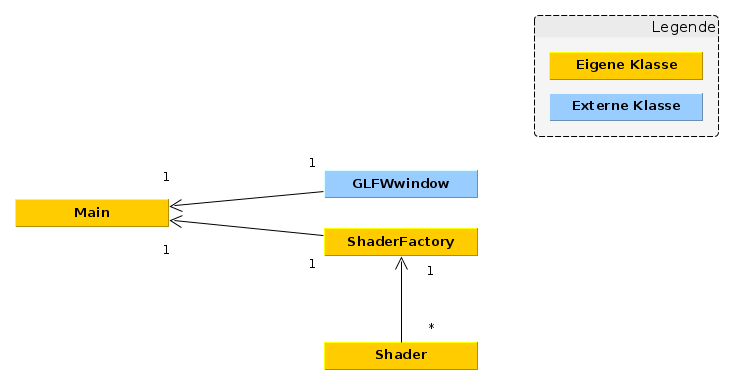
\includegraphics[width=0.8\textwidth]{img/prototype_class_diagram.png}
    \caption{Architektur des Prototypen\protect\footnotemark}\label{fig:prototype_architecture}
\end{figure}
\footnotetext{Eigene Darstellung mittels yEd.}

\subsection{Programmablauf}
\label{subsec:program_sequence}

Wie in Abbildung~\ref{fig:prototype_architecture} ersichtlich ist, besteht
die Applikation hauptsächlich aus der Hautpklasse. Diese initialisiert
mittels GLEW OpenGL und erstellt mittels GLFW ein Fenster sowie einen
OpenGL-Kontext. Danach wird eine Instanz des ShaderManagers erstellt,
welche ihrerseits alle verfügbaren GLSL-Shader in einem gegebenen
Verzeichnis lädt. Bei diesem Prototypen kommt jedoch nur ein Shader zum
Einsatz --- bestehend aus einem Vertex- sowie einem Fragment-Teil.

Die Applikation läuft danach in einer Endlosschleife, hört dabei aber
auf Events in Form von Keyboard-Eingaben. So kann die Applikation
jederzeit mit der Abbruch-Taste (ESC, Escape) beendet werden.

Die Hauptidee der Applikation ist die, dass diese im Rendering-Teil
einen Vertex- sowie einen Fragment-Shader lädt und ausführt. Der
Vertex-Shader tut nichts anderes als zwei Polygone in Form von Dreiecken
über die verfügbare Bildfläche darzustellen. Das eigentliche Rendering
von impliziten Oberflächen geschieht dann im Fragment-Shader. Dies ist
in der untenstehenden Abbildung~\ref{fig:prototype_shaders} verdeutlicht.

\begin{figure}[H]
    \centering
    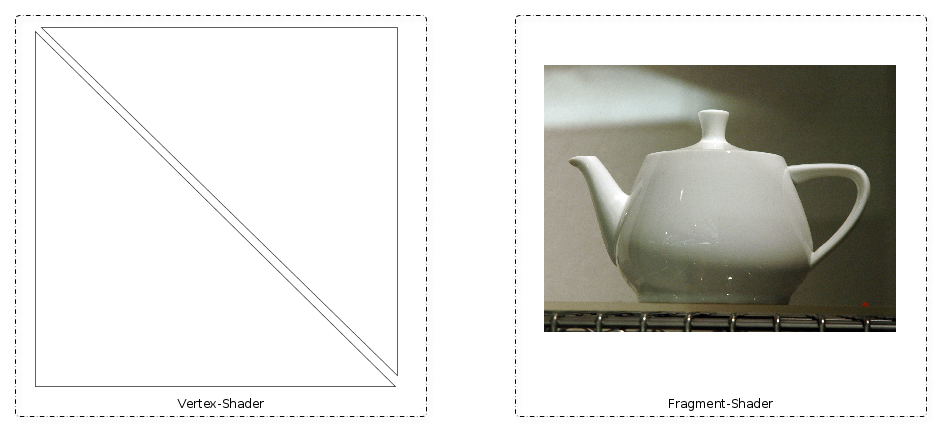
\includegraphics[width=0.8\textwidth]{img/prototype_shaders.png}
    \caption{Bildliche Darstellung der Funktionsweise von Vertex- und
        Fragmentshader der Applikation\protect\footnotemark}\label{fig:prototype_shaders}
\end{figure}
\footnotetext{Eigene Darstellung mittels yEd. Bei dem Bild des
    Fragment-Shaders handelt es sich um den so genannten ``Utah
    Teapot'', bezogen
    von~\url{http://www.flickr.com/photo_zoom.gne?id=352811902&size=o},
    alle Rechte für das Bild liegen bei Marshall Astor
    (\url{http://www.marshallastor.com/}).}

\section{Rendering}
\label{sec:rendering}

\todo[inline]{Describe rendering algorithm as it will be used in
    fragment shader}
